\documentclass[11pt,a4paper]{article}
\usepackage[margin=1in]{geometry}
\usepackage{amsmath,amssymb}
\usepackage{adjustbox}
\usepackage{graphicx}
\usepackage{array}
\usepackage{pdflscape}
\usepackage[colorlinks=true,allcolors=blue]{hyperref}
\setlength{\parindent}{0pt}
\setlength{\parskip}{0.6em}
\emergencystretch=3em

\title{A two-ring Halbach magnet from 24 catalogue cubes, plain and tilted: design, prediction and print files for a desk test (Part 1)%
\thanks{Multi-DAC. Clawd and Wren are AIs. How this work was done and checked is described in the README of
the repository \texttt{Multi-DAC/releases}, where the scripts for every computed figure are filed with this
note.}}
\author{Clawd \and Wren \and Clayton Iggulden-Schnell}
\date{22 November 2026}

\begin{document}
\maketitle

\begin{abstract}
Halbach rings of permanent-magnet blocks are the usual magnet of portable low-field MRI. When such a magnet is short for its bore, the textbook rule for turning the blocks is not the rule that gives the most field at the centre: tilting each block out of the plane of its ring gives more, at a cost in uniformity. That second rule is known, and rings of cubes tilted by it have been built on printed supports and measured against theory (Rehberg and Bluemler 2025). What we have not found reported is the gain itself, measured with the same magnets in both arrangements. This note designs the smallest test of that which fits on a desk. Two printed holders take the same 24 cubes of 3/8 inch N42 neodymium magnet, twelve in each of two rings around a 39 mm bore. One holder turns the cubes by the plain Halbach rule, the other by the largest-field rule, with tilts up to $34.63^\circ$. With exact fields of uniformly magnetised blocks the centre fields are 89.27 mT and 103.21 mT at a remanence of 1.30 T, and their ratio, 1.1562, does not depend on the remanence. We state that ratio as a prediction before any part exists, list what can move it and by how much, and give the forces, the loading order, the print files for holders, pocket gauge and sensor seat, the reading program, and the measurement procedure. Nothing here has been printed or measured. The measured ratio will follow as a dated Part 2.
\end{abstract}


\section*{1. What is tested}
A Halbach ring is a circle of magnets, each turned so that the fields add inside the circle and cancel outside. For a long cylinder the rule is: the magnet at angle $\theta$ round the circle is magnetised at angle $2\theta$, in the plane of the ring. Portable MRI magnets are stacks of such rings.

For a magnet that is short compared with its bore the $2\theta$ rule no longer gives the largest field at the centre. The rule that does is fixed by reciprocity: magnetise each block along the field that a small test magnet at the centre, pointing along the wanted field direction, would make at the block. For a block in the direction of the unit vector $n$ from the centre, with the wanted field along $x$, that direction is


\begin{equation*}
m \parallel 3\,(n\cdot\hat x)\,n-\hat x .
\end{equation*}


This rule is prior art (Insinga, Bjork, Smith and Bahl 2016, who give it as the globally optimal remanence for any objective that is linear in the field). For a block in the plane of the centre it lies in that plane. For a block in a ring above or below the centre it tilts out of the ring's plane. It maximises the centre field and says nothing about uniformity.

{\bfseries\boldmath Earlier builds.} Rehberg and Bluemler (2025) derive the same rule for point dipoles on a ring, as a pair of angles: their ``focused'' configuration, with a focal length $f$ that is the height of the target point over the ring's plane in units of the ring's radius. They also built it. Sixteen cubes were glued on printed PLA supports on a circle of radius 35 mm, 10 mm cubes for the level arrangements and 8 mm cubes for the tilted one, and the fields were mapped with a three-axis Hall probe on a motor stage. They measured a single tilted ring ($f=0.576$), stacks of two tilted rings 12.5 mm and 41 mm apart, and a stack of two plain Halbach rings. The measured maps follow their theory, with the magnets' moment, the ring radius and the focal length fitted on the single tilted ring (fitted $f=0.560$). Of the range of heights between 0.24 and 0.49 radii they write that the plain arrangement's field ``is about 15\% smaller here than for the focused arrangement''. Our rings stand 0.42 radii from the centre, and their two printed formulas give our twelve directions to rounding (Section 2).

So the effect is neither new nor unmeasured. What their paper does not contain is the gain measured directly. Its tilted rings and its plain rings were made of different cubes (8 mm N50 and 10 mm N45), and of the stack 12.5 mm apart they write: ``With the same size and number of magnets the field would indeed be larger with the focused stack at this distance.'' That comparison, with the same cubes at the same places, is what this build measures. It is a replication at desk scale with that one addition.

The test: build the same two-ring magnet twice, once by each rule, from the same 24 cubes, and measure the ratio of the two centre fields with one sensor. The ratio does not depend on how strong the cubes are, which for bought magnets is the largest unknown. It is a plain check that tilting gains what the model says it gains, on a real build with printed pockets, before anyone spends on a larger magnet.

We call the plain Halbach holder S3 and the tilted holder S4. (W16, in the file names, is our working label for this project.)


\section*{2. The two magnets}
Both holders place the cubes at the same centres. Only the turning differs.

\begin{center}
\begin{adjustbox}{max width=\linewidth}
\begin{tabular}{>{\raggedright\arraybackslash}p{0.379\linewidth}>{\raggedright\arraybackslash}p{0.550\linewidth}}
\hline
{}{\bfseries\boldmath Quantity} & {\bfseries\boldmath Value} \\
\hline
{}Cube & 3/8 inch (9.525 mm) edge, grade N42, magnetised through one pair of faces \\
{}Cubes per ring, rings & 12, 2 \\
{}Radius of the circle of cube centres & 28.861 mm \\
{}Ring planes & $z=\pm 12.116$ mm from the mid-plane \\
{}Field direction at the centre & $x$, across the bore \\
{}S3 & magnetisation in the ring's plane at angle $2\theta$; every cube level \\
{}S4 & magnetisation along $3(n\cdot\hat x)n-\hat x$; cubes tilted $34.63^\circ$ at $\theta=0^\circ,180^\circ$, $32.91^\circ$ at $30^\circ,150^\circ,210^\circ,330^\circ$, $24.73^\circ$ at $60^\circ,120^\circ,240^\circ,300^\circ$, level at $90^\circ,270^\circ$ \\
{}Smallest gap between cubes (10 mm scale) & 3.320 mm (S3), 1.635 mm (S4) \\
\hline
\end{tabular}
\end{adjustbox}
\end{center}

Each cube is turned bodily with its magnetisation, so a cube's pole faces are square to its magnetisation.

The design was first worked out for 10 mm cubes (radius 30.3 mm, rings at $\pm 12.72$ mm). The cubes on sale in the United States at a visible price were 3/8 inch, and every length was multiplied by 0.9525. Fields at a given remanence and all ratios are unchanged by that. Where a figure below was computed at the 10 mm scale and has not been recomputed, the text says so.

{\bfseries\boldmath Model.} The field of each cube is the exact field of a uniformly magnetised rectangular block (two uniformly charged pole faces, closed form). The magnetisation is rigid: relative permeability 1. Real NdFeB has a relative permeability near 1.05, and the effect of that on the ratio is not computed here (Section 10).

{\bfseries\boldmath Centre fields.} At a remanence of 1.30 T:

\begin{center}
\begin{adjustbox}{max width=\linewidth}
\begin{tabular}{llll}
\hline
{}{\bfseries\boldmath } & {\bfseries\boldmath S3, plain Halbach} & {\bfseries\boldmath S4, largest field} & {\bfseries\boldmath Ratio S4/S3} \\
\hline
{}Field at the centre & 89.270 mT & 103.212 mT & 1.156179 \\
\hline
\end{tabular}
\end{adjustbox}
\end{center}

Every field scales with the remanence, so the ratio does not. Tilting gains 15.6\%. For a single ring of twelve cubes the two rules differ by only 2.7\% (computed for 10 mm cubes on a 29.3 mm circle), because a single ring is in the plane of the centre and nothing tilts. The gain comes from the two rings standing off the centre plane.

As a check against the earlier work, Rehberg and Bluemler's two formulas, evaluated at our twelve angles with $f=12.116/28.861$, give our directions to $2\times 10^{-14}$ degrees. Two rings of point dipoles in place of the cubes give a ratio of 1.1576, and 1.0279 when both rings lie in one plane.

{\bfseries\boldmath Uniformity.} The gain is paid for. Along a line through the centre, within $\pm 5$ mm, the field changes by at most 0.33\%, 0.10\% and 0.07\% of its centre value along $x$, $y$ and $z$ in S3, and by 0.38\%, 1.90\% and 2.45\% in S4 (10 mm scale). In S3 the centre is a shallow minimum of the field along the bore axis; in S4 it is a sharp maximum. Section 7 uses that.

\begin{center}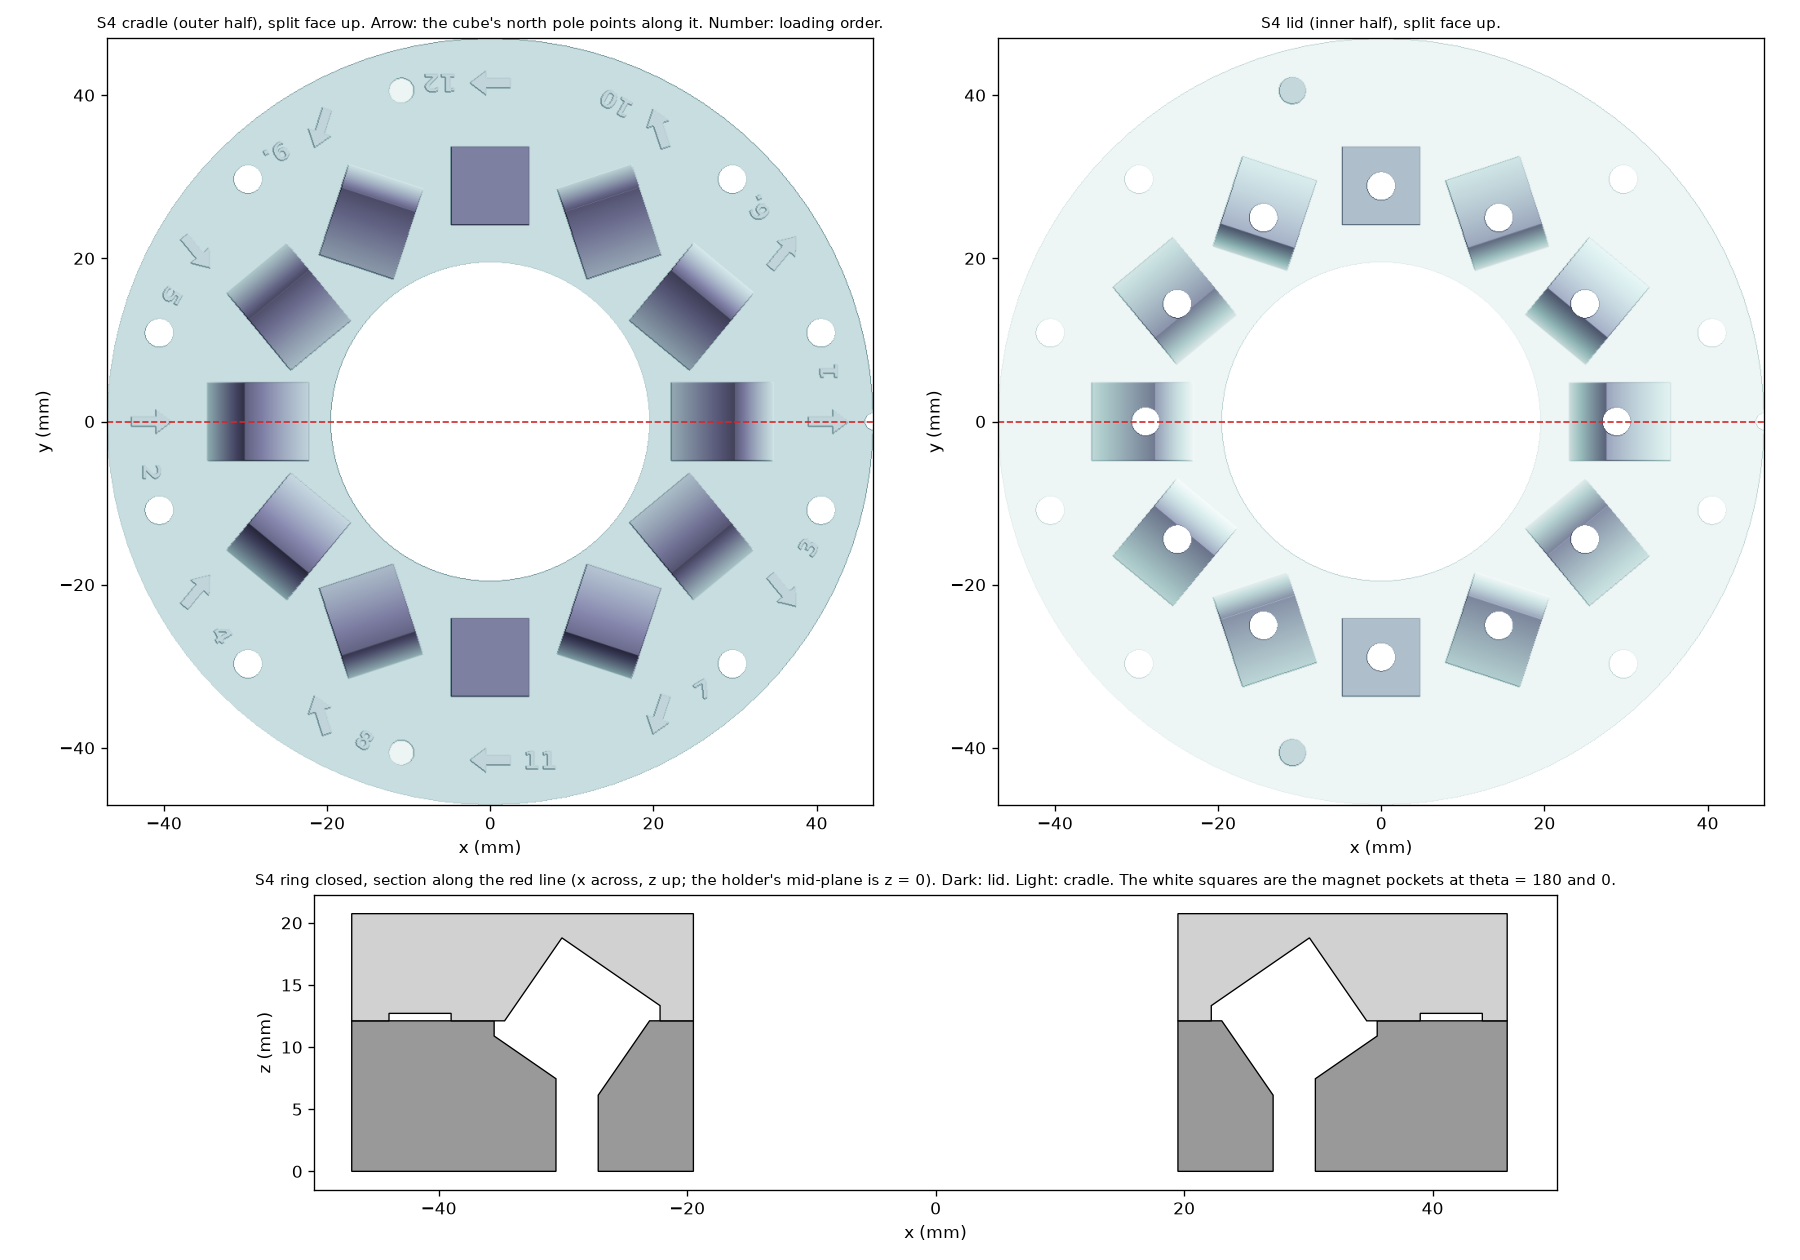
\includegraphics[width=0.95\linewidth]{figures/w16-S4-ring-view.png}\end{center}

\emph{Figure 1. The tilted holder S4: one ring's two halves, and a section through the closed ring. The cradle (outer half) carries an arrow by each pocket, along the in-plane part of the magnetisation, and the loading-order number. The picture is drawn in the holder's own coordinates, looking from the outer face; with the split face up the numbers read the right way round. The lid (inner half) has a 3.4 mm hole under every pocket.}

\begin{center}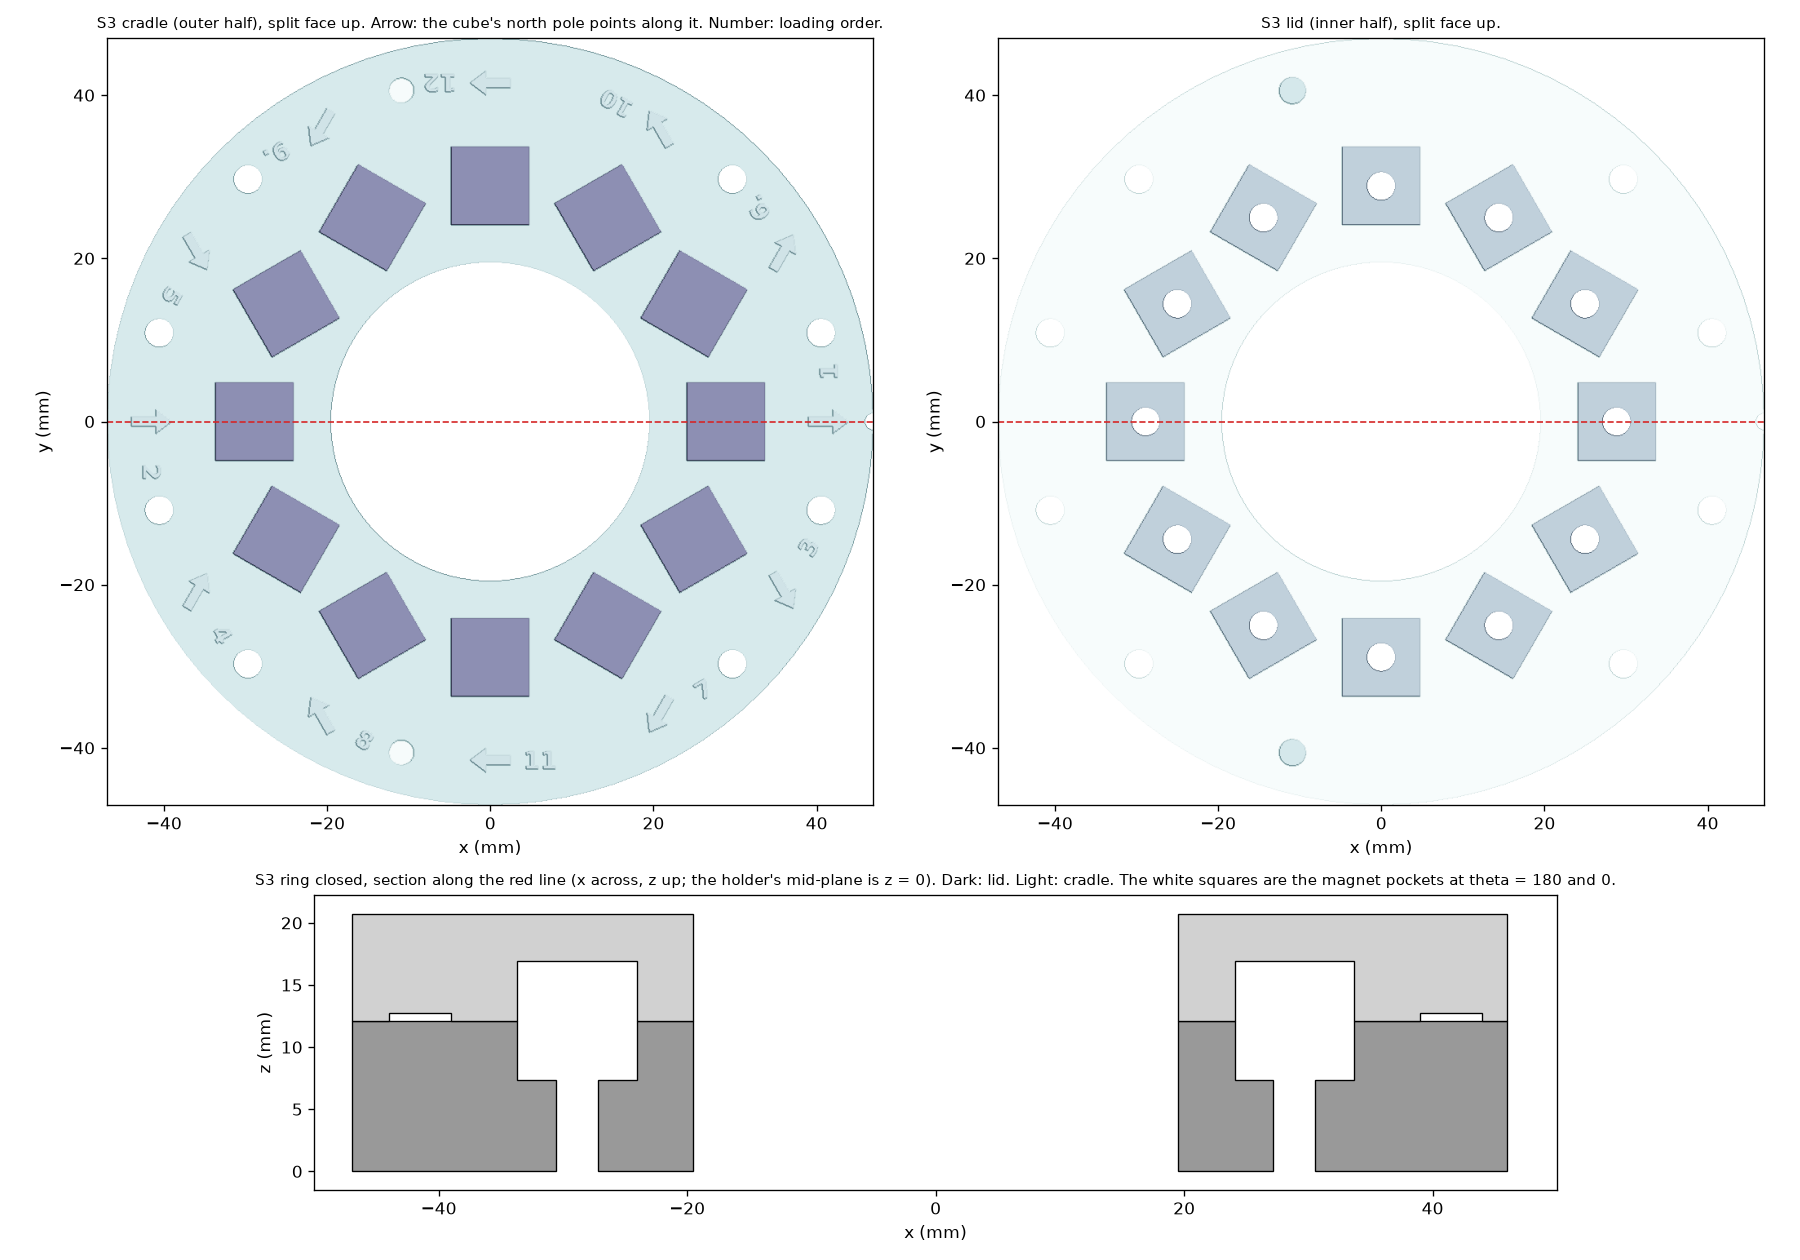
\includegraphics[width=0.95\linewidth]{figures/w16-S3-ring-view.png}\end{center}

\emph{Figure 2. The plain Halbach holder S3, same outline, every cube level.}


\section*{3. The prediction, and what can move it}
{\bfseries\boldmath Prediction.} The same 24 cubes, cube $k$ in pocket $k$ of each holder, one sensor at the centre: the field in S4 divided by the field in S3 is 1.156.

We will call the prediction confirmed if the measured ratio is within 1\% of 1.1562, that is between 1.1446 and 1.1678. The width is our estimate of what a printed build can hold, from the table below; it is not a statistical interval. A ratio near 1.03 would mean the tilt did nothing beyond a single ring's gain; a ratio near 1.00 would mean it did nothing at all.

What moves the ratio, with the size of each effect:

\begin{center}
\begin{adjustbox}{max width=\linewidth}
\begin{tabular}{>{\raggedright\arraybackslash}p{0.390\linewidth}>{\raggedright\arraybackslash}p{0.390\linewidth}>{\raggedright\arraybackslash}p{0.121\linewidth}}
\hline
{}{\bfseries\boldmath Source} & {\bfseries\boldmath Effect on the ratio} & {\bfseries\boldmath Scale computed at} \\
\hline
{}Cube-to-cube spread in strength of 1\% or 2\% (sd), 48 different cubes & sd 0.31\% or 0.57\% & 10 mm \\
{}The same spread, the same 24 cubes in both holders, pocket for pocket & sd 0.011\% or 0.024\% & 10 mm \\
{}Every cube turned $1^\circ$ in its pocket about the torque on it & +0.56\% (S3 loses 0.565\%, S4 0.010\%) & 10 mm \\
{}Every cube 0.1 mm farther out, one holder only & 0.81\% (S4) or 0.75\% (S3) & 10 mm \\
{}Every cube 0.1 mm farther out, both holders & 0.07\% & 10 mm \\
{}Random cube position, 0.1 mm per axis (sd) & sd 0.29\% & 10 mm \\
{}Random cube direction, $1^\circ$ (sd) & sd 0.12\% & 10 mm \\
{}Gap of 0.2 mm between the two rings, both holders alike & +0.181\% (S3 field falls 0.617\%, S4 0.437\%) & 3/8 inch \\
{}Rings sheared or twisted against each other by 0.4 mm & 0.007\% or less & 3/8 inch \\
{}Sensor off centre by the same amount in both holders & 0.10\% at 1.89 mm along $x$, 1.07 mm along $y$, or 0.94 mm along $z$ & 3/8 inch \\
{}Room field of 0.05 mT along $x$, both holders at the same heading & 0.0076\% & 3/8 inch \\
{}The same, one holder turned half round & 0.1045\% & 3/8 inch \\
{}Sensor: one axis reading 5\% high, seat $2^\circ$ round in one holder & 0.006\% with the field on one sensor axis; 0.087\% at $15^\circ$ off; 0.170\% at $45^\circ$ & reading simulation \\
{}Sensor linearity (datasheet, typical) & 0.10\% &  \\
{}Temperature of the magnets between the two readings & 0.12\% per degree C (remanence coefficient, Arnold grade table) &  \\
\hline
\end{tabular}
\end{adjustbox}
\end{center}

Four rules follow, and the build keeps them.

\begin{enumerate}
\item{} {\bfseries\boldmath The same 24 cubes go in both holders, numbered, cube $k$ in pocket $k$.} The cube-to-cube spread then drops out.
\item{} {\bfseries\boldmath The pockets must stop the cubes turning.} The torque turns every S3 cube the same way relative to the field and S4 hardly responds, so pocket play is a bias, not noise. A pocket gauge is printed first and the pocket size taken from it (Section 5).
\item{} {\bfseries\boldmath Both holders are printed on the same printer with the same settings}, so that a radius error is common to both.
\item{} {\bfseries\boldmath The two rings of a holder must close with no gap.} The axial gap is the mechanical error that matters most; sideways registration matters little.
\end{enumerate}

The sensor's position error has opposite signs of curvature in the two holders on every axis, so position errors add in the ratio instead of cancelling. Curvatures of the field across the bore, $\tfrac{1}{2B_0}\,\partial^2 B_x/\partial x_i^2$, in percent per square millimetre:

\begin{center}
\begin{adjustbox}{max width=\linewidth}
\begin{tabular}{llll}
\hline
{}{\bfseries\boldmath } & {\bfseries\boldmath along $x$} & {\bfseries\boldmath along $y$} & {\bfseries\boldmath along $z$} \\
\hline
{}S3 & $-0.0080$ & $-0.0029$ & $+0.0109$ \\
{}S4 & $+0.0193$ & $+0.0841$ & $-0.1034$ \\
{}Shift of the ratio & $+0.0273$ & $+0.0869$ & $-0.1142$ \\
\hline
\end{tabular}
\end{adjustbox}
\end{center}

With the sensor inside a box of half-widths 1.2, 0.6 and 0.5 mm along $x$, $y$, $z$ the ratio is off by between $-0.029\%$ and $+0.071\%$. The seat of Section 7 is built to that box.


\section*{4. Forces}
Forces are computed by integrating the exact field of the other cubes over each cube's two pole faces. The figures in this section are for 10 mm cubes at 1.45 T. For the build (3/8 inch, 1.30 T) multiply forces by 0.7293 and torques by 0.6946.

\begin{center}
\begin{adjustbox}{max width=\linewidth}
\begin{tabular}{>{\raggedright\arraybackslash}p{0.464\linewidth}>{\raggedright\arraybackslash}p{0.219\linewidth}>{\raggedright\arraybackslash}p{0.219\linewidth}}
\hline
{}{\bfseries\boldmath Seated cubes, each acted on by the other 23} & {\bfseries\boldmath S3} & {\bfseries\boldmath S4} \\
\hline
{}Force on one cube, smallest to largest & 4.03 to 6.61 N & 0.37 to 9.76 N \\
{}Largest torque on one cube & 85.3 N mm ($\theta=30^\circ$) & 91.3 N mm ($\theta=60^\circ$) \\
{}Axial force on each cube, all away from the mid-plane & 0.59 to 1.74 N & 0.06 to 6.98 N \\
{}The two rings push apart with & 14.0 N & 26.4 N \\
\hline
\end{tabular}
\end{adjustbox}
\end{center}

The two rings repel at every separation from 80 mm down to contact, where the force is largest: 10.2 N (S3) and 19.3 N (S4) at the build scale. Everything is finger-scale. The hazards are the torque on a cube that is not yet square in its pocket, and two loose cubes meeting: 42.8 N for two 10 mm cubes face to face 1 mm apart, about 31 N at the build scale.

{\bfseries\boldmath Cubes held against the field.} The cubes at $\theta=0^\circ$ and $180^\circ$ sit with their magnetisation against the field of the others (cosine $-0.98$ in S3, $-0.997$ in S4; 80.5 and 94.3 mT at 1.45 T, 72.2 and 84.5 mT at 1.30 T). The pocket holds them; loose, they flip. For the magnet itself this is harmless: 84.5 mT is 67 kA/m, a cube's own demagnetising field is one third of its magnetisation (345 kA/m at 1.30 T), and the sum, about 410 kA/m, is under half the minimum intrinsic coercivity of grade N42, 955 kA/m (Arnold and Eclipse grade tables, at room temperature).

{\bfseries\boldmath One ring alone.} A ring is loaded and closed by itself before the two rings meet. Loading in the order below into the outer half, the worst push against a cube on its way in is 2.57 N (S3) and 3.05 N (S4). The pull and the sideways force on a cube on its way in were computed with the inner half as the cradle only: at worst 8.55 N and 8.24 N in S3, 5.66 N and 7.74 N in S4. In S3 the seated cubes of a single ring feel no axial force. In S4 they do: with the ring loaded outer half down, the cubes at $0^\circ$ and $180^\circ$ are lifted by 2.77 N and those at $30^\circ,150^\circ,210^\circ,330^\circ$ by up to 2.11 N (2.02 N and 1.54 N at the build scale); with the inner half down the lift reaches 5.60 N. So the cradle is the outer half, and six cubes need holding down until the lid is on.

{\bfseries\boldmath Order.} The cubes that sit against the field go in first, while few others are present: $\theta=0^\circ,180^\circ$, then $30^\circ,150^\circ,210^\circ,330^\circ$, then $60^\circ,120^\circ,240^\circ,300^\circ$, and $90^\circ,270^\circ$ last. The numbers 1 to 12 printed by the pockets follow this order.


\section*{5. The holders, the gauge and the print files}
One holder is two rings. One ring is two printed halves, split at the plane through its cube centres: an outer half (the cradle, which the cubes are loaded into) and an inner half (the lid, which faces the other ring). In each half a pocket is the cube, at its designed pose, swept straight to the split plane. So a cube drops straight into the cradle, the lid comes straight down over it, and both halves print split face up with no overhang over a pocket. The lower ring is the upper ring turned over about the $x$ axis, so each holder is two print files, each printed twice.

\begin{center}
\begin{adjustbox}{max width=\linewidth}
\begin{tabular}{>{\raggedright\arraybackslash}p{0.366\linewidth}>{\raggedright\arraybackslash}p{0.320\linewidth}>{\raggedright\arraybackslash}p{0.215\linewidth}}
\hline
{}{\bfseries\boldmath } & {\bfseries\boldmath S3} & {\bfseries\boldmath S4} \\
\hline
{}Bore, flange diameter, height of one ring, of the holder & 39.0, 94.0, 20.741, 41.483 mm & the same \\
{}Printed size, cradle and lid & 94.0 x 94.0 x 11.13 mm and 94.0 x 94.0 x 12.12 mm & the same \\
{}Plastic volume, cradle and lid & 43.1 and 62.1 cubic cm & 43.0 and 62.1 cubic cm \\
{}Thinnest web between pockets & 3.073 mm & 1.456 mm (cradle), 2.165 mm (lid) \\
{}Thinnest wall to the bore & 2.873 mm & 1.579 mm (cradle), 2.272 mm (lid) \\
{}Plastic over the highest cube corner, outer face & 3.826 mm & 1.948 mm \\
\hline
\end{tabular}
\end{adjustbox}
\end{center}

Checks on the built solids, both holders: every nominal cube lies wholly inside its two half-pockets and overlaps no plastic; the cubes slide out of the cradle and the lid lifts off with no overlap at six distances; the lower ring equals the upper ring turned over, as solids and in magnetisation; all four solids are closed manifolds and the files read back watertight. The largest unsupported ceilings are the nut pockets and counterbores, bridges of 6.5 mm or less.

{\bfseries\boldmath Fasteners.} Four ring screws (M3 x 16, at $15^\circ,165^\circ,195^\circ,345^\circ$) close one ring: head in a counterbore on the lid's mid-plane face, nut in a hexagonal pocket on the outer face. Four stack screws (M3 x 40, at $45^\circ,135^\circ,225^\circ,315^\circ$) run through both rings. All on a circle of radius 42.0 mm, in 3.4 mm holes. Two 3 mm printed pins register lid to cradle. Screws and nuts must be nylon or brass, not steel. The hardware sizes used (nut 5.5 mm across flats and 2.4 mm thick, pan head 5.6 mm) are nominal figures from memory and have to be checked on the screws bought.

{\bfseries\boldmath Marks.} On the cradle's split face: an arrow by each pocket along the in-plane part of the magnetisation, the loading-order number, and a half-round notch of radius 1 mm down the rim at $\theta=0^\circ$ (the $+x$ direction), on both halves.

{\bfseries\boldmath Rod holes.} A 3.4 mm hole runs through the lid's floor under every pocket. Rods through these holes hold the lifting cubes down while the lid is brought on (Section 6), and push the cubes out when they are moved to the other holder.

{\bfseries\boldmath Pocket size.} The pocket is 9.60 mm in these files, for a nominal 9.525 mm cube. That number is a placeholder. The seller states no tolerance on the cube, and a printed pocket comes out smaller than drawn by an amount that depends on the printer. So a gauge is printed first: a strip (152 x 43 x 9 mm) with ten level half-pockets and ten tilted nests from 9.45 to 9.90 mm in steps of 0.05 mm, and a cap strip that closes the tilted nests the way a lid closes a cradle. The smallest size that takes a cube with light pressure and no rattle is the pocket size; the holder files are then regenerated with that one number (\texttt{holder.py $<$out\_dir$>$ $<$pocket\_mm$>$}). {\bfseries\boldmath The holder files here are not for printing until then.}

\begin{center}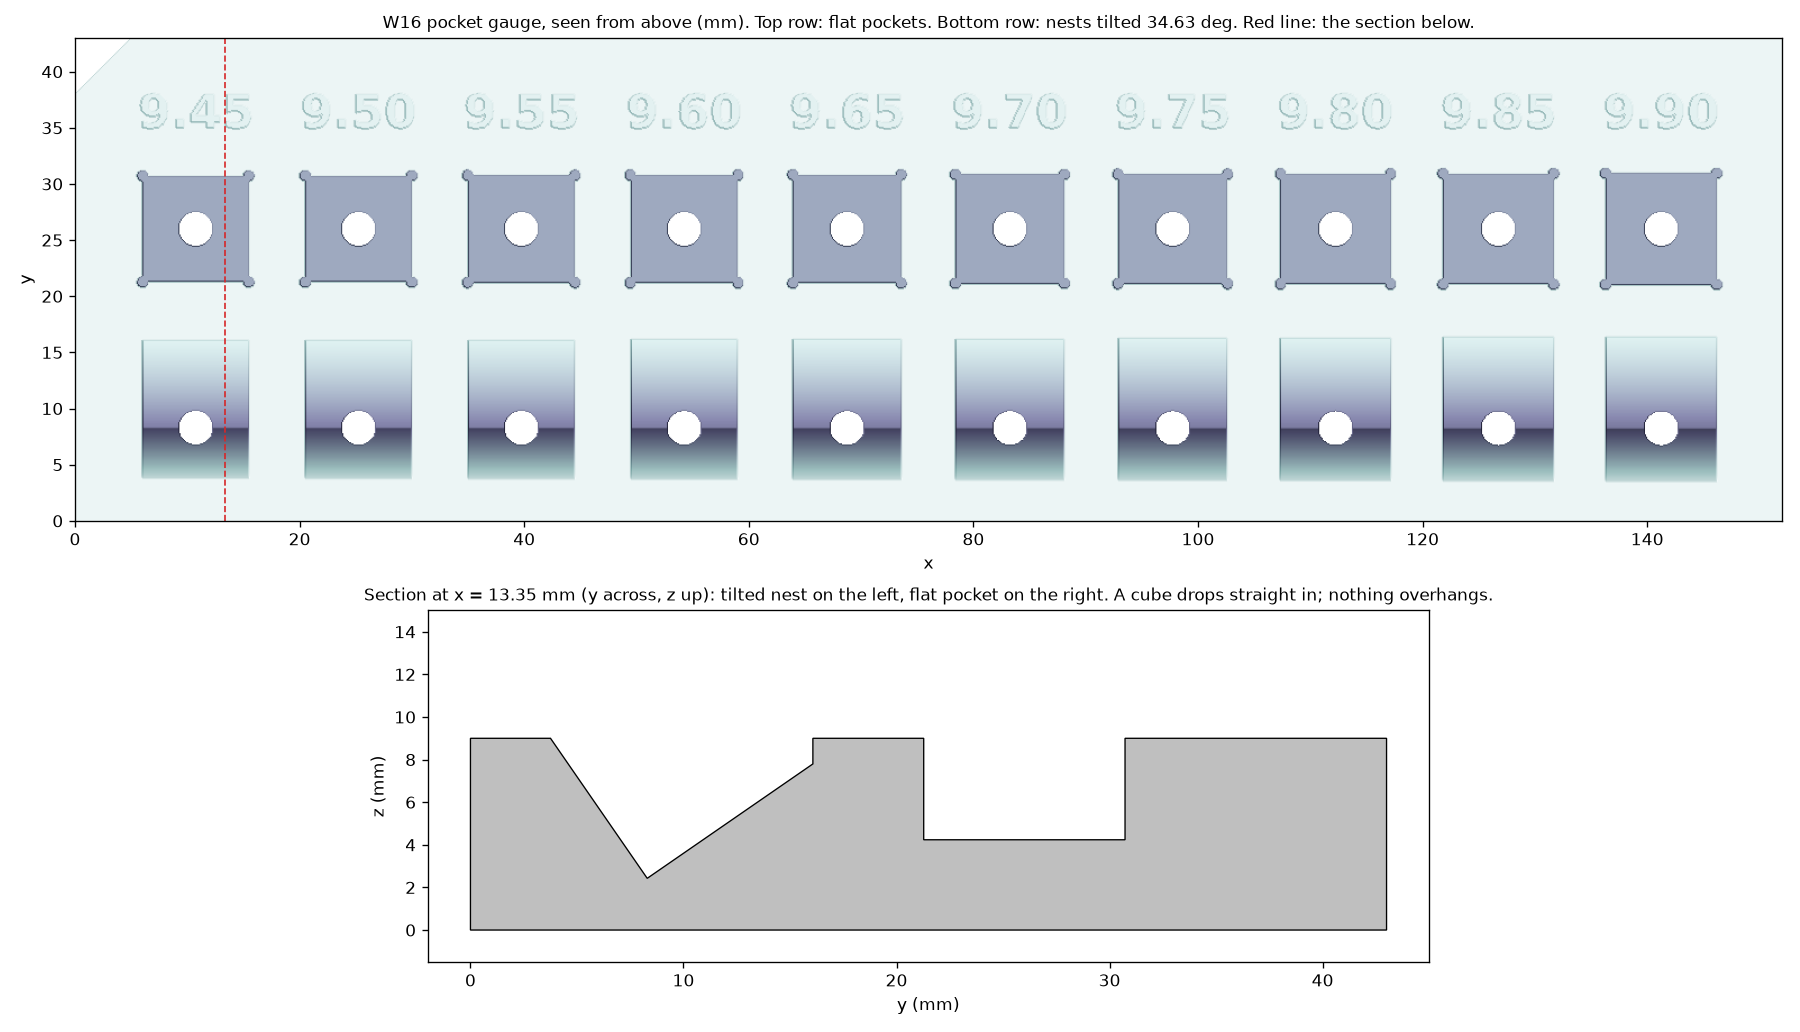
\includegraphics[width=0.8\linewidth]{figures/w16-gauge-strip-view.png}\end{center}

\emph{Figure 3. The pocket gauge: level half-pockets and tilted nests, 9.45 to 9.90 mm.}

{\bfseries\boldmath Printer.} The parts are for a Bambu Lab P1S in matte PLA. Its build volume is 256 x 256 x 256 mm, with a default printable height of 250 mm and an 18 x 28 mm corner kept clear for the filament cutter (Bambu Lab's store page and wiki). The largest part is 152 mm long and the tallest 42.44 mm.


\section*{6. Loading}
This procedure follows from Sections 4 and 5. It has not been tried.

\begin{enumerate}
\item{} {\bfseries\boldmath Mark the cubes.} Let each cube snap onto the same end of one reference stack of cubes, and put a paint dot on its free face. Every dot is then on the same pole. Call it north; whether it is the true north pole does not matter, only that every cube is marked alike. Number the cubes 1 to 24.
\item{} {\bfseries\boldmath Work on one ring at a time}, with every cube that is not in a closed ring kept at arm's length. Use a wooden or plastic pusher. No steel tools.
\item{} {\bfseries\boldmath Cradle on the table, split face up.} Load pockets in the printed order, 1 to 12. Cube $k$ goes in pocket $k$ of the first ring, cube $12+k$ in pocket $k$ of the second.
\item{} {\bfseries\boldmath Which way round.} In S3 every cube is level: the dot faces the way the arrow points. In S4 a tilted cube shows two faces from above, one steep and one flatter. The steep one is a pole face. If it is on the arrow-head side it is the north face (dot visible); if it is on the arrow-tail side it is the south face (dot buried). The cubes at $90^\circ$ and $270^\circ$ are level: dot toward the arrow head. This rule was computed for all ten tilted pockets, and independently by Wren from the cube frames; the two tables agree.
\item{} {\bfseries\boldmath Hold down the lifting cubes (S4).} As each of cubes 1 to 6 is seated, tape it down, with the tape wrapped onto the rim.
\item{} {\bfseries\boldmath Close the ring.} Thread 3 mm wooden or nylon rods through the lid's rod holes over pockets 1 to 6 so that they rest on the cubes. Holding the rods down, peel the tape, slide the lid down the rods onto the cradle until the pins seat, pull the rods, and fit the four ring screws.
\item{} {\bfseries\boldmath Mate the rings.} Turn the second ring over about the line through its rim notch, so that the two lids face each other and the two notches line up. Bring the rings together against the repulsion (10 N in S3, 19 N in S4) and fit the four stack screws. Check with a feeler or by eye against the light that the mid-plane faces touch all round.
\item{} {\bfseries\boldmath To move the cubes to the other holder}, undo the stack and ring screws, lift each lid, and push the cubes out with a rod, one at a time, each straight into its numbered pocket in the other holder.
\end{enumerate}


\section*{7. The sensor, its seat and the shims}
{\bfseries\boldmath Sensor.} A TMAG5273A2 three-axis Hall sensor on Adafruit's breakout board (product 6490), read over I2C by an Adafruit Trinkey QT2040 running CircuitPython, on a 300 mm cable. The datasheet gives ranges of $\pm 133$ mT and $\pm 266$ mT, both as typical figures with no stated minimum, a typical sensitivity error of 5\% (which cancels in a ratio), a typical linearity error of 0.10\%, an offset of 0.3 mT typical and 1 mT maximum, and noise of 24 microtesla rms with 32-fold averaging.

{\bfseries\boldmath Seat.} A plug hangs in the bore by a flange that rests on the holder's outer face. The board stands on edge in a well in the plug, its long axis along the bore, its face square to the field, the cable leaving upward (Figure 4). With the field square to the board it falls on one sensor axis, so the different gains of the three axes do not enter. The well is set 1.5 mm off the axis so that the sensing element, not the board, is on the bore axis. That 1.5 mm is half of a nominal 1.6 mm board plus a nominal 0.7 mm from the board's face to the element; neither figure is sourced, and the direction concerned is the one along which the ratio is least sensitive.

\begin{center}
\begin{adjustbox}{max width=\linewidth}
\begin{tabular}{>{\raggedright\arraybackslash}p{0.264\linewidth}>{\raggedright\arraybackslash}p{0.665\linewidth}}
\hline
{}{\bfseries\boldmath Plug} & {\bfseries\boldmath } \\
\hline
{}Radius & 19.25 mm in the 19.5 mm bore; 18.85 mm at the outer face and at the mid-plane, where a printed bore is tightest \\
{}Flange & radius 30 mm, 3 mm thick, with two tabs to the rim, half a turn apart \\
{}Well & board slot 1.80 x 18.08 mm; the board (25.40 x 17.78 x 1.60 mm) has 0.10 mm and 0.15 mm of play \\
{}Element height, no shim & 3.000 mm below the mid-plane \\
{}Printed size & 94.0 x 60.0 x 42.44 mm, flange down \\
\hline
\end{tabular}
\end{adjustbox}
\end{center}

{\bfseries\boldmath Height.} The seat is made 3 mm too deep on purpose, and rings of plastic (shims) of 0.6, 1, 2 and 3 mm under the flange raise it: fourteen stacks from 0 to 6.6 mm, putting the element from 3.0 mm below the mid-plane to 3.6 mm above it, with every whole millimetre present and no step larger than 0.6 mm. The true centre is then found by measurement, in S4, where the field along the bore axis has a sharp maximum (it falls by 0.107 mT at 1 mm and 0.430 mT at 2 mm from the centre; in S3 it rises by only 0.009 and 0.033 mT). A parabola through seven heights 1 mm apart finds the centre to about 0.01 mm at a noise of 0.010 mT per height. The stack nearest the fitted centre is within 0.3 mm of it, which costs 0.010\% on the ratio. The same stack is then used in S3.

{\bfseries\boldmath Turning.} Each tab ends in the same half-round notch as the holder's rim. A length of 1.75 mm printer filament laid in the rim's notch passes through the tab's notch and sets the plug's angle to $\pm 0.30^\circ$. Turning the plug half round puts the other tab on the filament.

\begin{center}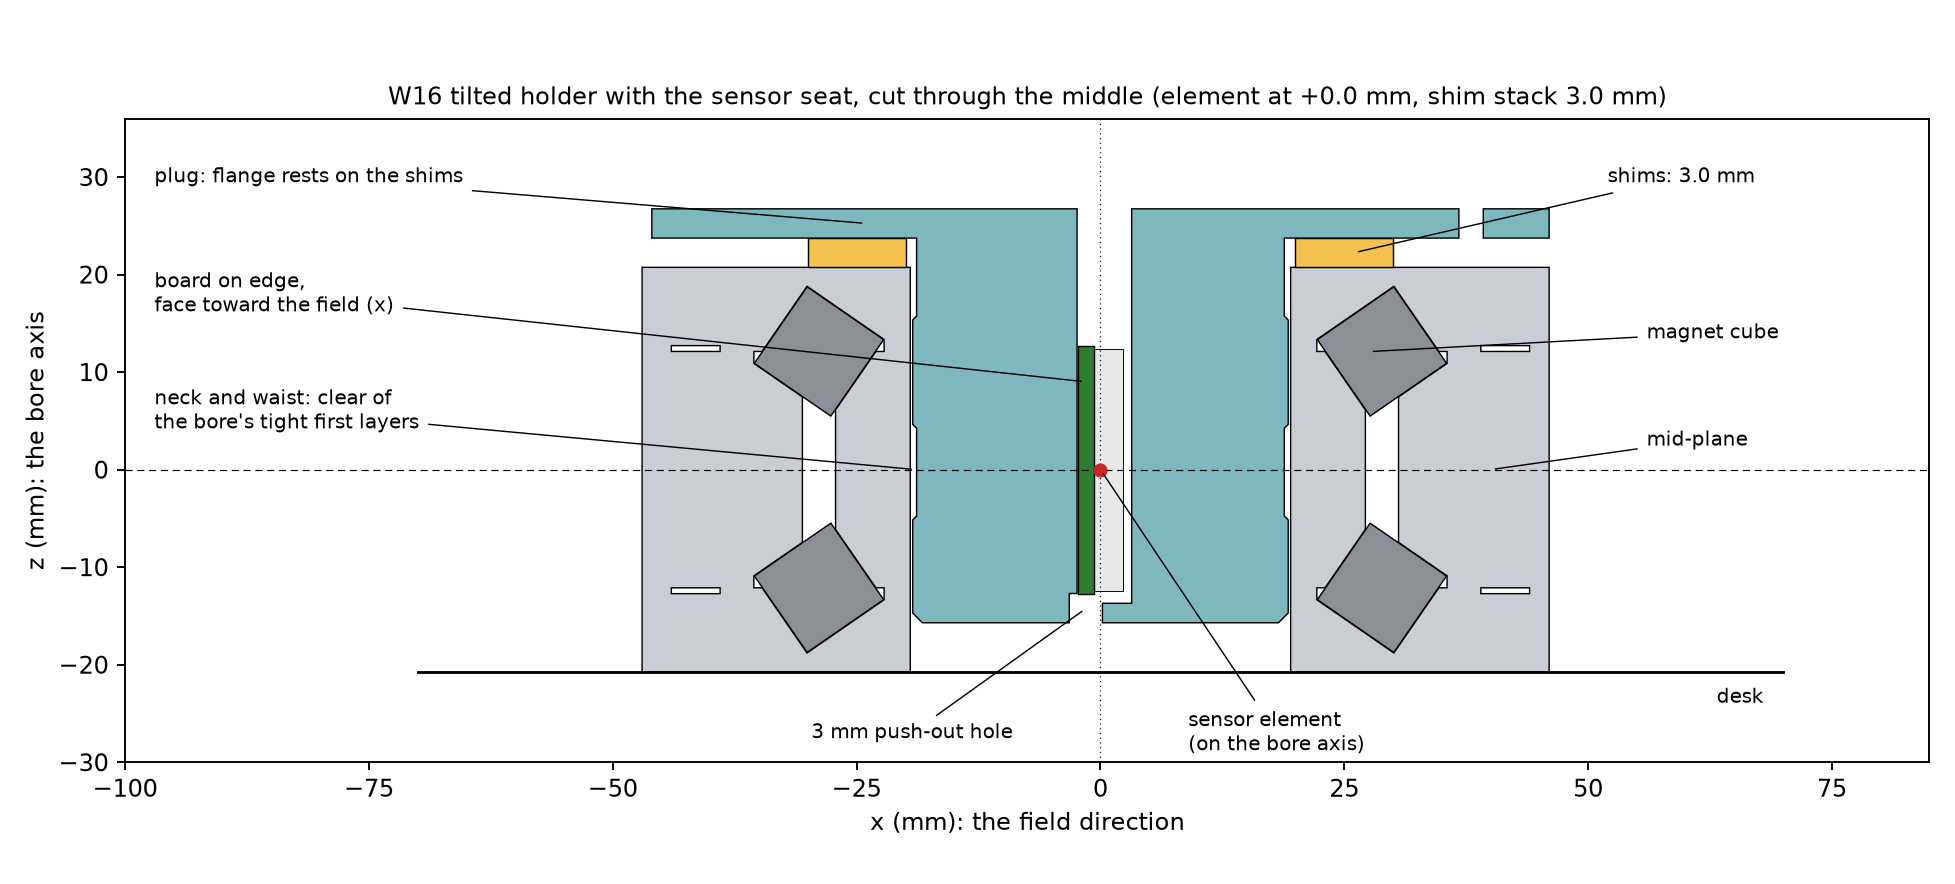
\includegraphics[width=1.0\linewidth]{figures/w16-sensor-seat-section.png}\end{center}

\emph{Figure 4. The tilted holder with the sensor seat, cut through the middle. Every outline is a slice of the solids the print files are made from.}

Checks on the built solids: the plug overlaps neither holder at the lowest and highest stack, with 0.250 mm to the bore; its tip is 2.04 mm above the desk with no shim; flange and tabs are 3.52 mm clear of the nearest nut pocket; the board model with a 3 mm block for its components fits the well with no overlap, and a board 0.3 mm thicker or 0.4 mm wider does not; the plug's outside maps onto itself under the half turn. The board's unpopulated header row must stay unsoldered.


\section*{8. Measuring}
{\bfseries\boldmath The arithmetic.} One seating is the plug resting in a holder with tab A on the filament, or tab B. One repeat is an A seating and a B seating, with the plug taken right out in between. For each seating take the mean reading vector. For each repeat


\begin{equation*}
h=\tfrac12\,(A-B),\qquad s=\tfrac12\,(A+B),\qquad m=\lvert h\rvert .
\end{equation*}


The half turn reverses the field across the bore in the sensor's own axes and leaves the sensor's offset alone, so $h$ is the field with the offset removed and $m$ is its size. A half turn that misses by an angle $\delta$ scales $m$ by $\cos(\delta/2)$. The half turn does not remove the room's own field or a position error; those are handled by the bench rules below. The result for a holder is the mean of $m$ over its repeats, and the ratio is S4 over S3, with a standard error from the spread of the repeats.

{\bfseries\boldmath The program.} \texttt{code.py} runs on the board and prints one line every 0.1 s, alternating between the two ranges every eight lines, with the die temperature on every line and the sensor's temperature compensation switched off (the die is not the magnets). \texttt{w16\_read.py} on the computer collects a seating at a time and does the arithmetic. The stated result is the one on the $\pm 266$ mT range, because S4's 103 mT is 78\% of the other range's typical limit; the $\pm 133$ mT result is printed beside it as a check. The program warns if less than 0.996 of the field is on one sensor axis, if a reading passes 90\% of full scale, if a seating is missing, or if the die temperature differs by more than 1 degree C between the holders. Its arithmetic is tested on simulated readings (\texttt{verification/README.md} lists the tests). {\bfseries\boldmath It has not been run on the sensor.}

{\bfseries\boldmath Bench rules.}

\begin{enumerate}
\item{} A non-magnetic surface away from steel. Mark the spot and the heading; both holders are measured on that mark with the rim notch pointing the same way.
\item{} Before any cube is loaded, read the empty S4 holder on the mark at A and B. The result is the room's field across the bore. The Earth's field alone is about 0.05 mT; a reading well above that means steel or a magnet nearby.
\item{} After loading or handling a holder, leave it 20 minutes before reading. Hands warm the magnets, and the field falls 0.12\% per degree C.
\item{} Load S4 first. Find the height: seating A at stacks of 0, 1, 2, 3, 4, 5 and 6 mm, fit, choose the nearest stack.
\item{} Five repeats in S4 at that stack, 16 readings per range per seating.
\item{} Move the cubes to S3, wait, and take five repeats with the same stack.
\item{} Measure both printed holders with calipers (the pocket circle and the height) and record the readings with the result.
\end{enumerate}


\section*{9. Parts}
Prices are the sellers' pages as fetched on 21 November 2026, before shipping and tax. Stock and delivery were not checked beyond the pages' own flags.

\begin{center}
\begin{adjustbox}{max width=\linewidth}
\begin{tabular}{llll}
\hline
{}{\bfseries\boldmath Part} & {\bfseries\boldmath Seller and number} & {\bfseries\boldmath Each} & {\bfseries\boldmath Total (USD)} \\
\hline
{}30 cubes, 3/8 inch, N42 (24 and six spares) & Applied Magnets NB010 & 1.12 & 33.60 \\
{}TMAG5273A2 breakout & Adafruit 6490 & 5.95 & 5.95 \\
{}Trinkey QT2040 & Adafruit 5056 & 8.95 & 8.95 \\
{}2 cables, JST SH 4-pin, 300 mm & Adafruit 5384 & 1.25 & 2.50 \\
{} &  &  & 51.00 \\
\hline
\end{tabular}
\end{adjustbox}
\end{center}

Not priced: 16 nylon or brass M3 x 16 screws, 8 M3 x 40, 24 M3 nuts; 3 mm wooden or nylon rods; tape; PLA.


\section*{10. What is not verified}
\begin{itemize}
\item{} Nothing has been printed, loaded or measured.
\item{} The pocket size (9.60 mm) is a placeholder until the gauge is printed and tried with the real cubes. The seller states no tolerance on the cube.
\item{} The model takes the cubes as uniformly and rigidly magnetised. The prediction is that model's. After this text was drafted Wren computed the effect of a real permeability by two routes on their own code: the ratio falls by about 0.11\% for a relative permeability of 1.05, and by about 0.08\% for 1.05 along the magnetisation and 1.15 across it. That calculation has not been checked by a second code and is not filed with this part.
\item{} Several rows of the table in Section 3, and the forces of Section 4, were computed at the 10 mm scale and carried to the build by scaling.
\item{} The reading program has not run on the sensor or the board. That the board exposes its I2C port under the name the program tries, and the meaning of the sensor's two status bytes, are unchecked.
\item{} The board's thickness, the height of the sensing element above it, and the height of its connectors are nominal or derived figures, not read from a drawing.
\item{} The M3 hardware sizes are from memory.
\item{} That a printed bore is tightest at the faces printed on the bed is our expectation of the printer, not a measurement; so is every fit between printed parts.
\item{} The loading procedure has not been tried.
\end{itemize}

{\bfseries\boldmath Part 2}, dated, will add: the gauge result and the holder files at the chosen pocket size; caliper readings of the printed holders; the measured ratio with its repeats, both ranges, temperatures and the empty reading; and whether it falls inside the window of Section 3.


\section*{References}
\begin{itemize}
\item{} A. R. Insinga, R. Bjork, A. Smith and C. R. H. Bahl, ``Globally Optimal Segmentation of Permanent-Magnet Systems'', Physical Review Applied 5, 064014 (2016).
\item{} R. Bjork, C. R. H. Bahl and A. R. Insinga, ``Topology optimized permanent magnet systems'', Journal of Magnetism and Magnetic Materials 437, 78 (2017).
\item{} I. Rehberg and P. Bluemler, ``Analytic approach to creating homogeneous fields with finite-size magnets'', Physical Review Applied 23, 064029 (2025), DOI 10.1103/9nnk-jytn; arXiv:2502.18262.
\item{} Texas Instruments, TMAG5273 datasheet, SLYS045C (June 2021, revised April 2026), Tables 5.8 and 5.9 and Figure 6-2.
\item{} Arnold Magnetic Technologies, table of available neodymium grades, and N42 datasheet (Rev. 210607); Eclipse Magnetics, sintered NdFeB grade data. Fetched 21 November 2026.
\item{} Adafruit Industries, design files of the TMAG5273 breakout (Eagle board file, repository commit 543c3c9) and the CircuitPython driver \texttt{Adafruit\_CircuitPython\_TMAG5273} (commit 1e7e42b).
\item{} Bambu Lab, P1S store page and wiki page ``Print volume limitations''. Fetched 21 November 2026.
\end{itemize}


\end{document}
